\documentclass{article}
\usepackage{main}

\title{Le paradoxe de Simpson}
\date{11 Octobre 2024}
\author{TSTMG2}

\begin{document}
\maketitle

On s'intéresse au lien entre activité sportive et réussite scolaire. Pour se faire, on a interrogé des élèves de deux classes d'un lycée à propos :
\begin{itemize}
\item du nombre d'heures consacré par semaine au sport;
\item et de leur moyenne en cours.  
\end{itemize}
Les résultats sont représentés sur ce graphique en nuage de points.
\begin{center}
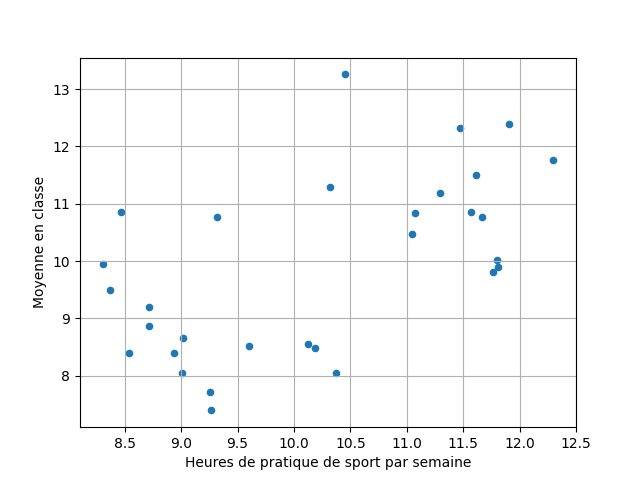
\includegraphics[width=\textwidth]{Global.png}
\end{center}
\paragraph{Questions}
\begin{enumquestions}
\item Quelle est environ la moyenne du plus sportif de ces élèves ?
\item Quelle est la pratique de sport de l'élève ayant la moyenne la plus basse ?
\item La phrase \og une grande pratique du sport améliore la moyenne\fg vous semble-t-elle justifiée ? Justifier à l'aide d'une droite d'ajustement.
\item On représente à la suite le même sondage, mais en choisissant une couleur différente pour chaque classe (Jaune pour terminale, et bleu foncé pour les secondes). Tracer la droite d'ajustement pour chacune des classes. Que remarquez-vous ? 
\end{enumquestions}
\begin{center}
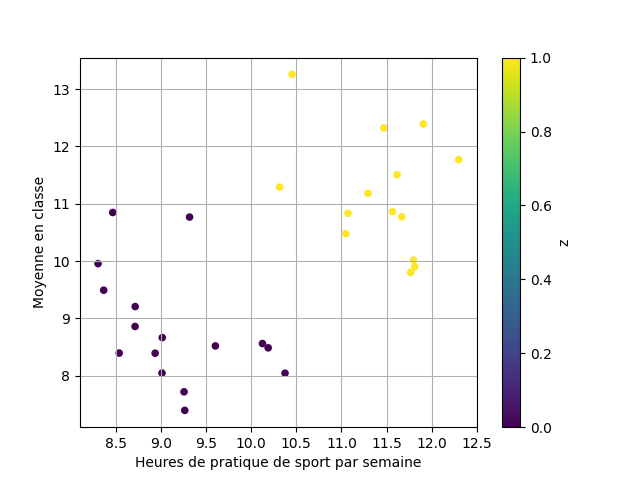
\includegraphics[width=\textwidth]{Local.png}
\end{center}
\end{document}